\documentclass[a4paper]{article}

%% Language and font encodings
\usepackage[english]{babel}
\usepackage[utf8x]{inputenc}
\usepackage[T1]{fontenc}
\usepackage{subfig}
\usepackage{multirow}
\usepackage{array}
\usepackage[noend]{algpseudocode}
\usepackage{algorithm}
\usepackage{pdfpages}
\usepackage{amsmath}


%% Sets page size and margins
\usepackage[a4paper,top=3cm,bottom=2cm,left=3cm,right=3cm,marginparwidth=1.75cm]{geometry}

%% Useful packages
\usepackage{amsmath}
\usepackage{graphicx}
\usepackage[colorinlistoftodos]{todonotes}
\usepackage[colorlinks=true, allcolors=blue]{hyperref}

\newcommand\descitem[1]{\item{\bfseries #1}\\}

\def\infinity{\rotatebox{90}{8}}
\def\hatz{\hat{z}}
\def\hatn{\hat{n}}
\def\pr{\mbox{P}}
\def\ex{\mbox{E}}
\def\leafsize{M_\bot}
\def\CB{{\cal B}}
\def\CT{{\cal T}}
\def\CM{{\cal M}}
\def\Node{\mbox{\sf Node}}

\title{Detecting Communities In Graphs with Highly Overlapping Communities using Bloom Filters}
\author{Pratham Shah \and Shubham Jain}

\begin{document}
\maketitle

\begin{abstract}
    Community detection is an interesting problem in the area of social networks. It gives us useful insights into the underlying structure of complex networks. Detection of communities in graphs can be a challenging task, and it poses an even bigger challenge if the graph has overlapping communities. In this report, we present an algorithm which detects local communities in graphs with overlapping communities. We use Bloom Filters to reduce memory footprint on the main memory.
\end{abstract}

\section{Introduction}
 Community in a network is a subset of nodes that are more densely than the rest of the network. Community detection is an interesting problem in the area of social networks. It gives us useful insights into the underlying structure of complex networks. There exist algorithms which give good results in finding communities in graphs when the communities are not overlapping \cite{lancichinetti:2008} \cite{PRN}. However, community detection is a challenge when the graph has overlapping communities. 
 
In this report, we present an algorithm which detects local communities in graphs with overlapping communities. We use Bloom Filters to reduce memory footprint on the main memory.


\section{Preliminaries}


\subsection{Bloom Filters}
Bloom Filters \cite{Bloom:1970:STH:362686.362692} were introduced by B. H. Bloom in 1970. It is a space-efficient data structure that answers set-membership queries with some false positive rate. They have found numerous applications due to their tremendous space-efficient nature.

\subsection{Bloom Sample Trees}
A Bloom Sample Tree \cite{sengupta:2017} is a novel data structure that can be used to perform multiple operations involving Bloom Filters. A Bloom Sample Tree organises the namespace like a binary search tree. Each node is a Bloom Filter that contains a subset of the namespace. Union of all the Bloom Filters at a level yields the entire namespace. We use Bloom Sample Trees here to sample multiple elements from Bloom Filters and to calculate the set difference between two Bloom Filters.


\subsubsection{Sampling From Bloom Filter}
We extend the method provided in \cite{sengupta:2017} and use threads to sample multiple elements from a Bloom Filter. \newline
Given a Bloom Filter $B$ to sample $n$ elements from, we proceed in the following recursive fashion to get $n$ samples elements:
\newline
\begin{itemize}
    \item Create a Bloom Sample Tree with the namespace of the Bloom Filter.
    \item At a given (non-leaf) node, compute the intersection of the Bloom filters stored in the left and right children of this node with $b$. If for both child nodes, the intersection is empty, then $b$ does not contain any element belonging in the range associated with this node. Therefore the subtree rooted at this node is pruned from the search. 
    \newline
    The estimated number of elements in the intersection of two Bloom filters $\CB_1$ and $\CB_2$ is given by the following expression \cite{Papapetrou2010}:
$$
\hat{S}^{-1} ( t_1, t_2, t_{\wedge} ) = 
\frac{
    \ln{\left(  m - \frac{t_{\wedge} \times m - t_1 \times t_2}{m - t_1 - t_2 + t_\wedge} \right) - \ln(m)}
}
{
    k \times \ln \left(1 - \frac{1}{m} \right)
}
$$
where $t_1$ is the number of bits set in $\CB_1$, $t_2$ is the number of bits set in $\CB_2$, $m$ is the size of both Bloom filters, $k$ is number of hash functions used in both, and $t_\wedge$ is the number of bits set in the bitwise AND of $\CB_1$ and $\CB_2$. 

\item If intersection with only one child is non-empty, then a new thread is created to proceed the search along that child node. The other child node and the subtree rooted at it are pruned from the search.

\item If intersection with both child nodes is non-empty, then two threads are created, one for proceeding the search along the left subtree and the other to carry the search along the right subtree. The number of elements to be sampled from the right and left child nodes is proportional to the number of elements in their respective intersections. Note that it is possible that the intersection was a false positive and this is discovered further down this subtree. In that case, the search then backtracks and proceeds along the other child node.


\item At a leaf node, every element in the range of the node is checked for membership in $b$. The samples at this leaf node are sampled uniformly at random from the set of values that satisfy the membership test of $b$. If none of the elements within this range satisfies the membership query, it indicates that the search has reached this leaf node due to a (string of) false set overlap(s). In this case, the sample at this node is $NULL$.

\end{itemize}




One another approach to sample elements from a Bloom Filter using a Bloom Search Tree is to create a thread pool. A fixed number of threads are created. To sample $n$ elements, a job queue is created, and the task is added to the job queue. Whenever a thread is idle in the thread pool, it fetches a job from the job queue and samples an element independently.
\newline

\textbf{Experimental Analysis} 
We used a static synthetic namespace to compare the running time of the different approaches. We varied our namespace from $10^5$ to $10^7$. We also varied the number of samples to be generated from $1000$ to $10000$. In the combined approach, we have used 256 threads for the below experiments. In the experiments we performed; we generated query sets uniformly at random from the entire namespace. We compared the running time of both the approaches listed and compared it to the running time of generating a single sample, the required number of times. \newline


\textbf{Results}
Figure 1 shows the average time taken to sample multiple elements from a set using a Bloom Sample Tree using different approaches. The experiment demonstrate that creating multiple threads in advance and then using each to handle multiple nodes is the best strategy of the proposed ones. $Multithreading$ refers to the approach where we create a new thread at each node and distribute the task among children of a node. $Thread pool$ refers to the approach where we create $256$ threads and use a job queue to sample elements.
\begin{figure}[h!] 
\centering
\begin{tabular}{cccc}
\subfloat[$m=10^4$, $n=10^4$, $M=10^5$]{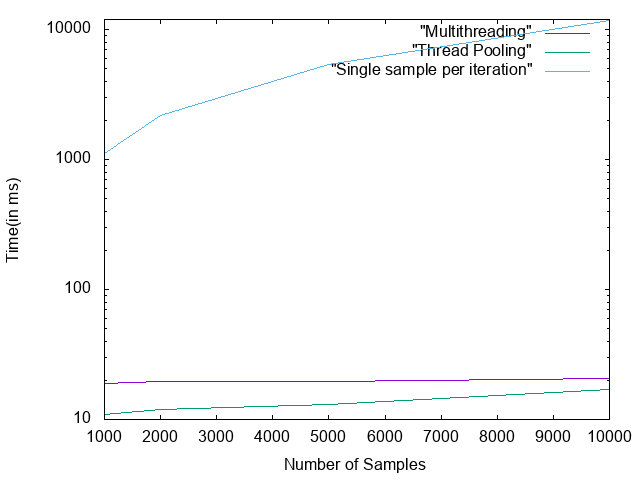
\includegraphics[width=0.5\textwidth]{plot5.png}} 
\subfloat[$m=10^5$, $n=10^4$, $M=10^6$]{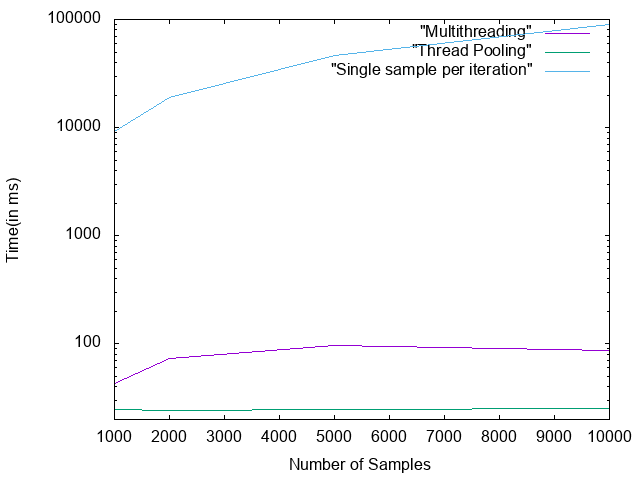
\includegraphics[width=0.5\textwidth]{plot6.png}}\\
\subfloat[$m=10^6$, $n=10^4$, $M=10^7$]
{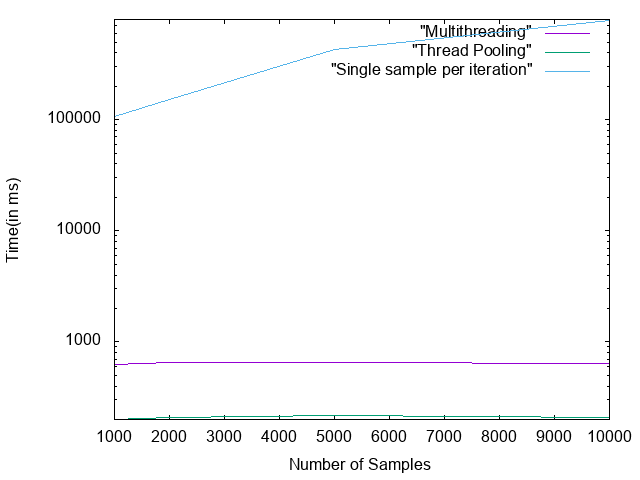
\includegraphics[width=0.5\textwidth]{plot7.png}}
\subfloat[$m=10^6$, $n=10^4$, $M=10^8$]
{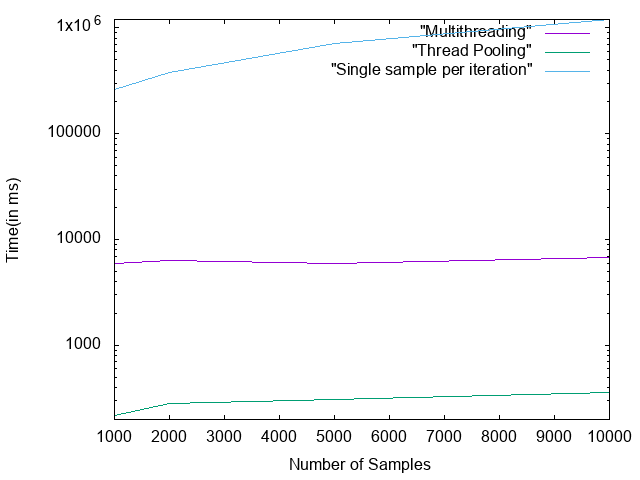
\includegraphics[width=0.5\textwidth]{plot8.png}}
\end{tabular}

\caption{\label{fig:plot}Time taken for different approaches}
\end{figure}

\subsubsection{Calculation of Set Difference Between Two Bloom Filters}
In this section, we give a method to estimate elements in the set difference between two sets represented as Bloom Filters. \newline
\textit{Problem Statement}. If we are given two sets $S1$ and $S2$ from a namespace $U$ stored in Bloom Filters $B1$ and $B2$ respectively, then we try to estimate elements that are in $S1$ but not in $S2$. \newline
$Solution Overview.$ We exploit Bloom Sample Tree \cite{sengupta:2017} to represent the entire namespace. We go down the tree estimating the number of common elements between nodes of the tree and $S1$ and $S2$. If no common element with $S1$ is found, search along that path is pruned, if no common element with $S2$ is found, the node is added into the result and if there are common elements with both sets are found, we move a level down on the path.


\begin{algorithm}
\caption{$Set\_diff (B_{ij}, S, C)$}
\begin{algorithmic}[1]
\Procedure{Set\_diff}{$B_{ij}, S, C$}
 \If{$isLeaf(B_{ij})$}
    \State \textbf{return} all elements of $B_{ij}$ that are in $S$ and not in $C$
  \ElsIf{$B_{ij} \cap S = \phi$}
    \State  \textbf{return} $\phi$
     \ElsIf{$B_{ij} \cap C = \phi$}
    \State  \textbf{return} $S$
    \Else 
    \State
    \textbf{return} $Set\_diff (B_{i+1,2j}, S, C) \cup Set\_diff (B_{i+1,2j+1}, S, C)$
  \EndIf
\EndProcedure
\end{algorithmic}
\end{algorithm}
\begin{algorithm}
\caption{$Set\_difference (B_{ij}, S, C)$}
\begin{algorithmic}[1]
\Procedure{Set\_difference}{$B_{ij}, S, C$}
 \State 
 \textbf{return} $Set\_diff (B_{0,0}, S, C)$
\EndProcedure
\end{algorithmic}
\end{algorithm}




\begin{figure}[h!] 
\centering
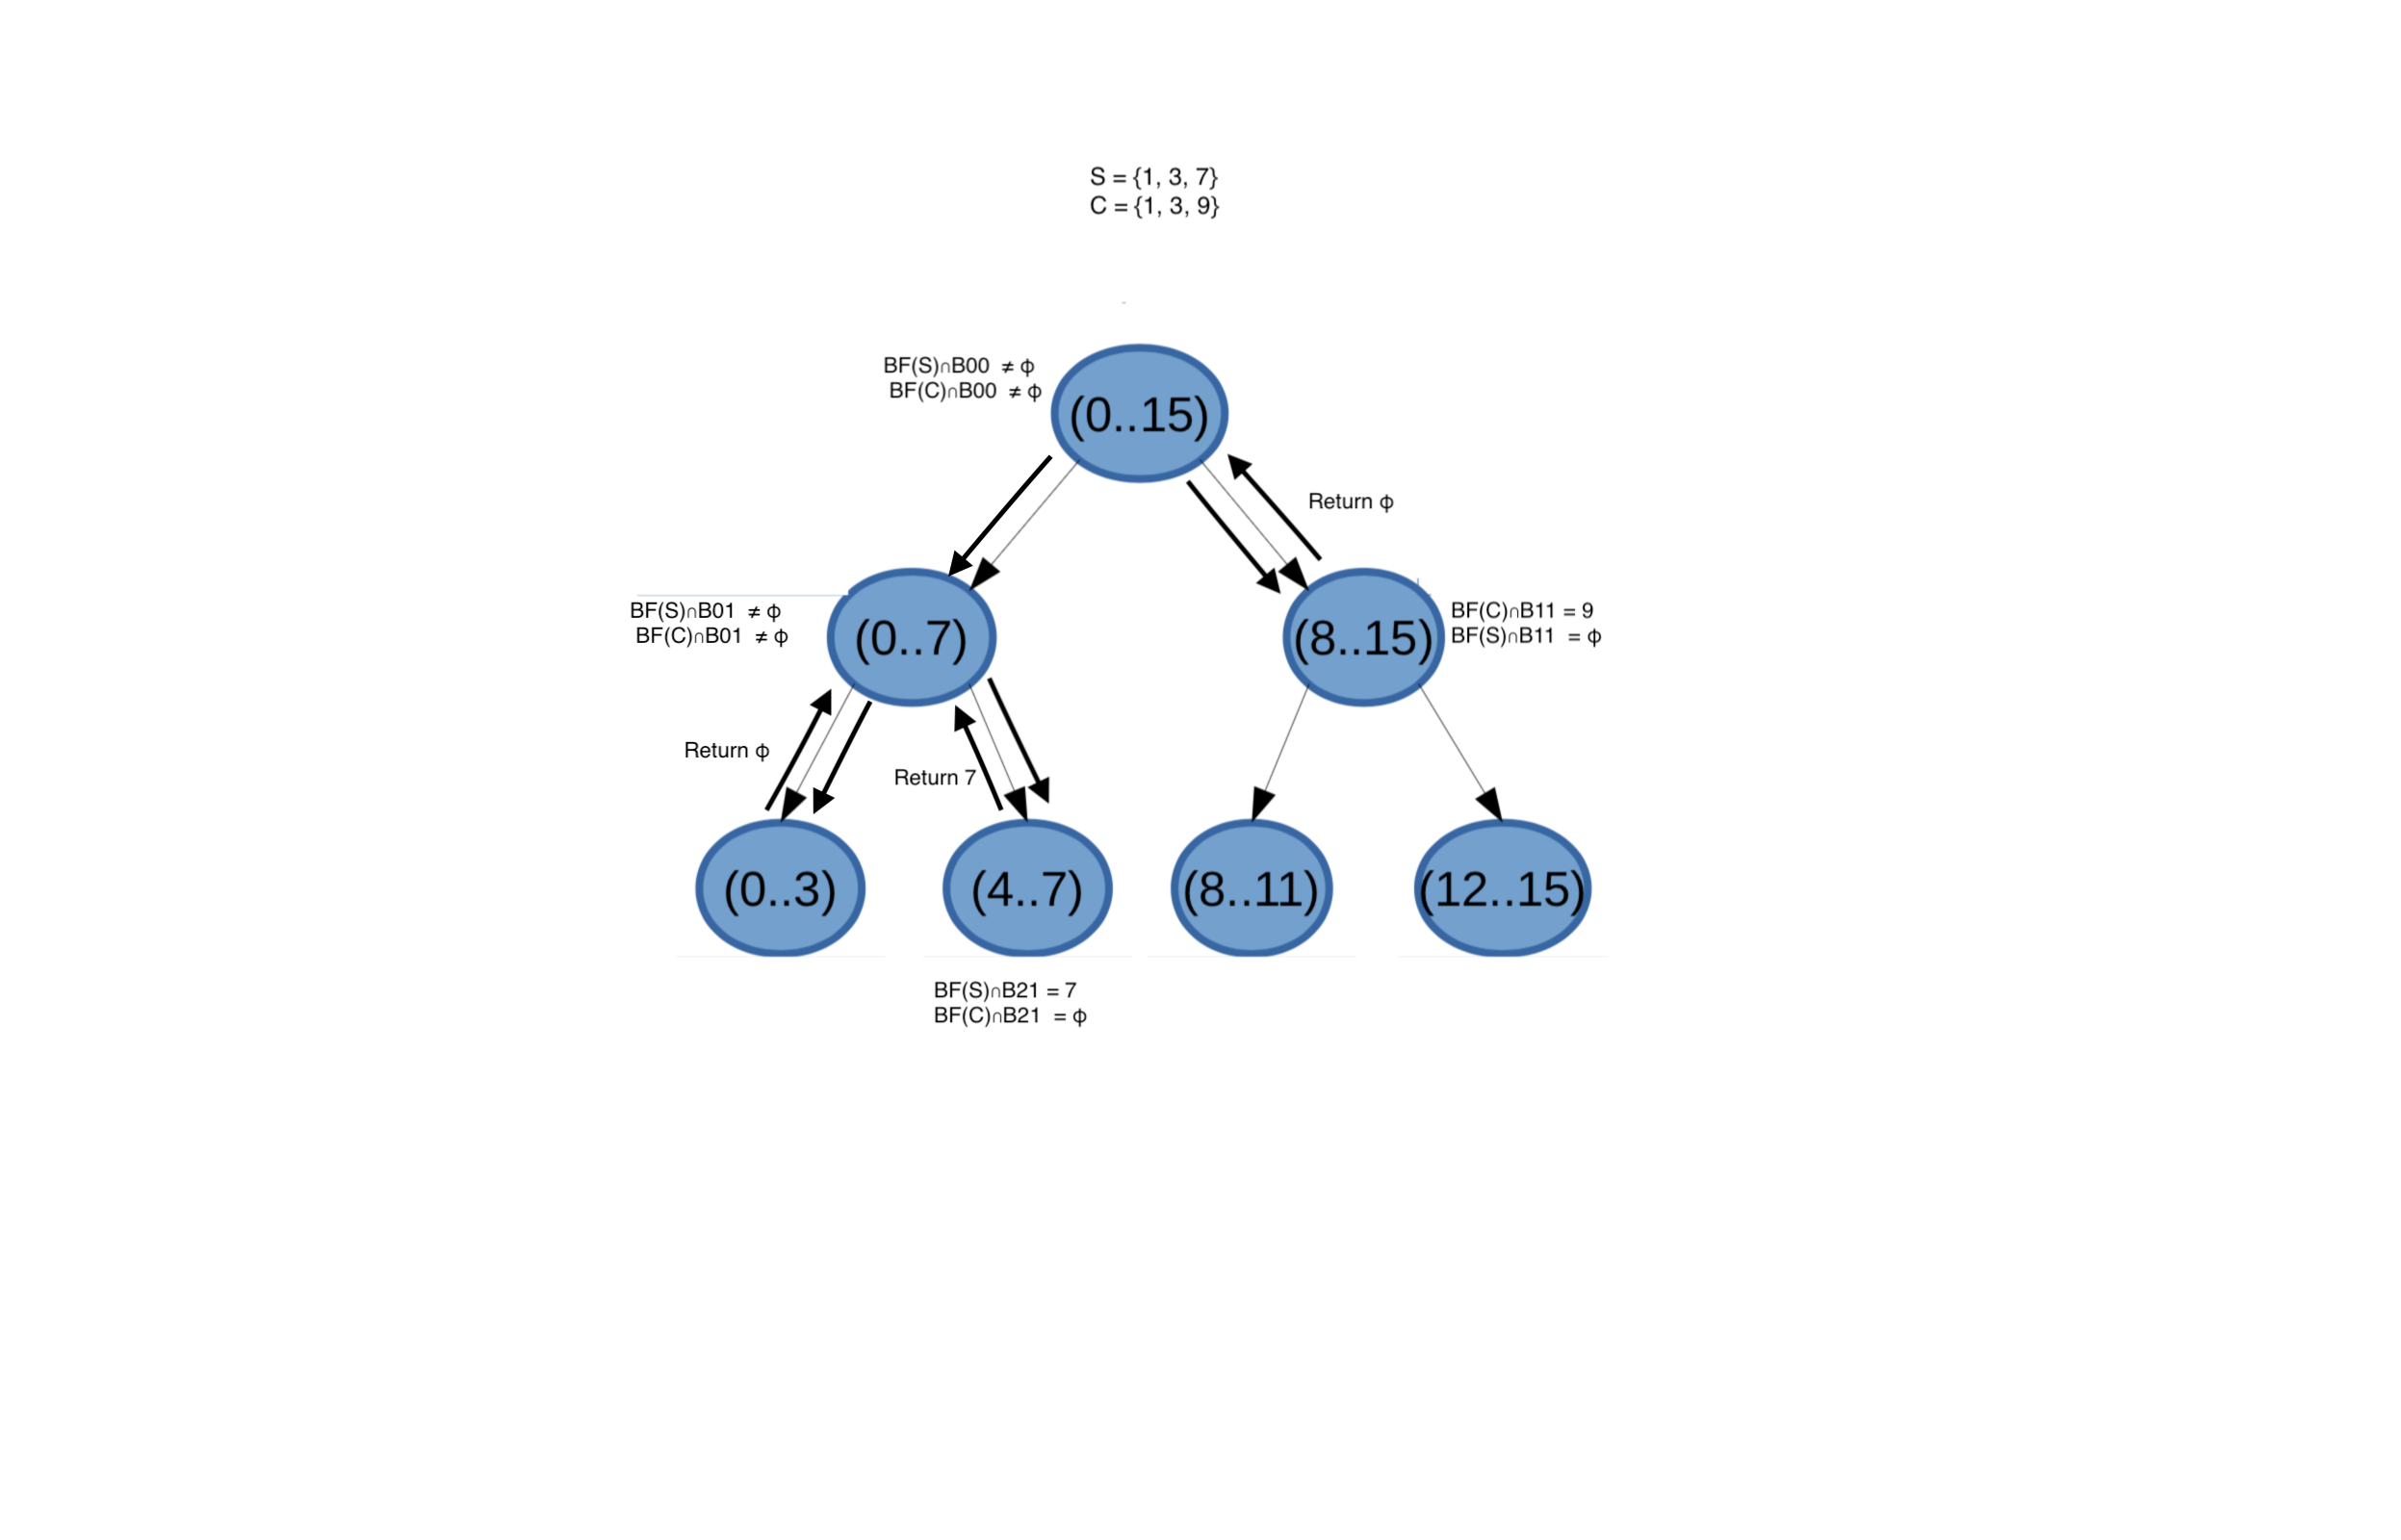
\includegraphics[width=0.6\textwidth]{sd.png}
\caption{\label{fig:Set Difference}Calculation of set difference}
\end{figure}


\textbf{Experimental Analysis}
We use a synthetic namespace $M$ (=$[1, 2, 3, ... 10^6]$). The Bloom Filter size is $50,000$. Both sets $A$, and $B$ are sampled uniformly at random without replacement from $M$.
Initially, the size of $B$ is fixed to $500$, and the size of $A$ is varied in $(10,20,40,80,160,320,640,1280)$.
 Similarly, later, the size of $A$ is fixed to 500, and the size of $B$ is varied in the same set.
 
 
$A-B$ was calculated independently keeping the sizes of one set constant and varying the other. Precision, recall and F1-score were calculated for the experiments
\textbf{Results}
 Figure 3 describes precision, recall and F1-score variation in calculating the Set difference between two sets.

\begin{figure}[h!] 
\centering
\begin{tabular}{cccc}
\subfloat[$A-B$ with varying $B$ and constant $A$]
{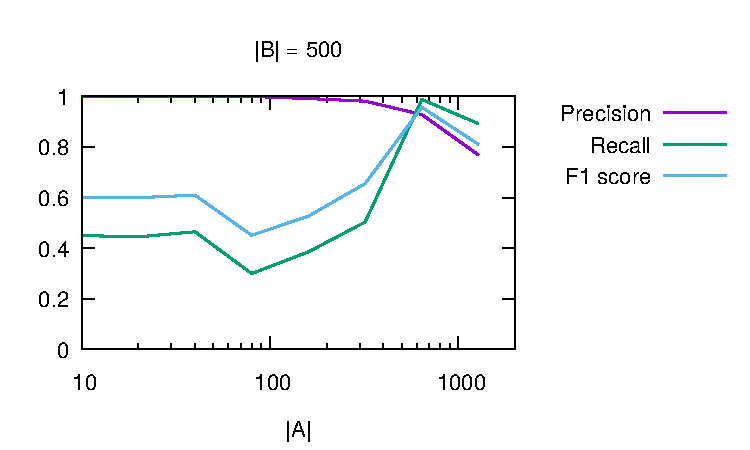
\includegraphics[width=0.5\textwidth]{AResults.pdf}} 
\subfloat[$A-B$ with varying $A$ and constant $B$]
{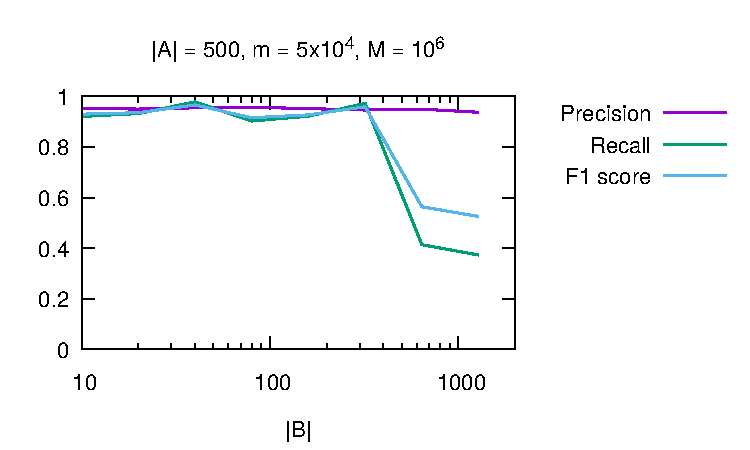
\includegraphics[width=0.5\textwidth]{BResults.pdf}}
\end{tabular}

\caption{\label{fig:plot}F1-score for Set difference}
\end{figure}







\section{Detection of Communities in Graphs with Overlapping Communities}


Communities are a significant part of many networks like social networks as they tell about relationships between different people in the network. In the real world, it can be seen that a single entity may belong to multiple communities. Thus, it can be an important problem to find communities in graphs with overlapping communities. \newline

One might find it useful use Bloom Filters as a storage data structure because of their space-efficient nature. 

\textit{Problem Statement}. \cite{Wu2012} describes the community detection formally as: Given an undirected network $G$ = ($V, E$) where $V$ represents the set of vertices in the graph and $E$ the set of edges, we have perfect knowledge of the connectivity of some set of vertices, i.e., the known local community of the graph, which is denoted as $C$. Necessarily, a set of vertices $N$ that are adjacent to vertices in $C$ but do not belong to $C$ can be partially known (note “partially” means that the complete connectivity of any vertex in $N$ is unknown). Moreover, we define the shell vertex set as region $S$, where any vertex $v \epsilon S$ has at least one neighbour in $N$. Let assume that the only way to gain further knowledge about $G$ is to choose one vertex from $N$ and merge it into $C$. Thus the additional unknown vertices may be added to $N$. The task of this problem is to constitute a local community $C$ from a single source vertex by this one-vertex-at-a-time step.\newline


\textit{Solution Overview}. Given an undirected network G = (V, E) where V represents the set of vertices in the graph and E the set of edges. Let us denote shell nodes as set S and community node as set C.Any vertex v $\epsilon$ S has at least one neighbour in C and v $\not\in$ C. \newline
To detect communities, we are going to expand around a seed node. The algorithm uses a fitness measure. Fitness Measure value describes how well-connected community is. The algorithm only adds those nodes one-by-one to the community which increases community fitness. We stop when an addition of no node increases the fitness function\newline


\textit{Alpha-Measure}\cite{lancichinetti:2008}. It is a community fitness measure we used in our algorithm for measuring community fitness.\newline
$K_{in}$ denotes the sum of in-degree and out-degree of the nodes in the community.
$K_{out}$ denotes the sum of out-degree of the nodes whose one end of the edge is in the community, and another end is connected with a node outside community.\newline
$\alpha$ is a hyper-parameter which can be adjusted accordingly.

\begin{align*}
F_S 
&= \frac{k_{in}^S}{(k_{in}^S+k_{out}^S)^\alpha}  
\end{align*}





\subsection{Algorithm}

The algorithm to generate communities from a graph containing communities with highly overlapping communities can be summarized as follows:
\begin{enumerate}
    \item Initialize shell and community as empty bloom filters.
\item Select a seed, push it and its neighbors into the community and shell bloom filters respectively.
\item Sample some nodes from the shell, and choose the node which results in highest community fitness.
\item Push the node found in above step and push it into the community.
\item  Update the shell as set difference of shell and community.
\item Repeat 3-5 until no node is found which increases the community fitness.



\end{enumerate}


The following is the formal algorithm. \textit{seed} refers to initial seed for the procedure, $\alpha$ is the hyper-parameter $\alpha$ to be used for $\alpha\_measure$ and $k$ is the number of elements to be sampled from the $shell$ Bloom Filter.
 
\begin{algorithm}
\caption{$Community\_detection (seed, k, \alpha)$}
\begin{algorithmic}[1]
\Procedure{Community\_detection}{seed, k}
\State $ community\gets seed$        \Comment{Community Bloom Filter}
\State $ shell\gets adj(seed)$        \Comment{Shell Bloom Filter}
\State $ size\gets 1$
\State $ k_{in} \gets 0$
\State $ k_{out} \gets |adj(seed)|$
\State $ \alpha\_measure\gets 0$ 
\While{True}
\State $candidate\_list\gets sample(shell, k)$\Comment{Sample $k$ elements from the $shell$ Bloom Filter}
\State $node \gets NULL$
\State $save_{in}\gets -1$
\State $save_{out}\gets -1$
\For{$v \epsilon candidate\_list$}
\State $x_{in}\gets 0$


\For{$z \epsilon adj(v)$}          \Comment{Add comment here}
\If{$is_in(community, z)$}          

\State $x_{in} \gets x_{in}+1$

\EndIf
\EndFor

\State $x_{out} \gets |adj(v) - x_{in}|$
\State $temp_{in} \gets k_{in}+2*x_{in}$
\State $temp_{out} \gets k_{out}-x_{in}+x_{out}$
\State \alpha\_measure\_temp \gets  $temp_{in}$/{($temp_{in}$+$temp_{out}$)^\alpha}

\If{$\alpha\_measure\_temp > max$}
\State $max\gets \alpha\_measure\_temp$
\State $node \gets v$
\State $save_{in} \gets temp_{in}, save_{out} \gets temp_{out}$
\EndIf
\EndFor

\If{$max > \alpha\_measure$}
\State $\alpha\_measure \gets max$
\State $community \gets community \cup node$ 
\State $shell \gets Set\_diff(shell, community)$
\State $k_{in} \gets save_{in}, k_{out} \gets save_{out}$
\Else \State break
\EndIf
\EndFor
\EndWhile
\State \textbf{return} $community$
\EndProcedure
\end{algorithmic}
\end{algorithm}




\subsection{Experiments and Results}

In our experiments, we compare the results of the following algorithms:
\begin{enumerate}
    \descitem{LFM} This is a basic algorithm described in \cite{lancichinetti:2008}. It also uses the \textit{Alpha Measure}.
    \descitem{PRN} This algorithm is described in \cite{PRN}.
    \descitem{GCE} This algorithm finds cliques in the graph and finds communities around those cliques as seeds. It is described in \cite{1002.1827}.
    \descitem{GCE Local} It is a local version of GCE that we implemented so that results can be compared. It can be described as follows. Given seed node $s$, collect all neighbors of $s$ = $N$. Find cliques in the subgraph induced by $N$. i.e. the subgraph that has only the nodes in $N$, and any edges of the graph that are between nodes in $N$. Expand cliques using the clique expansion algorithm \cite{1002.1827}.

    \descitem{1 node expansion} We expand community using a seed node. We sample neighbouring nodes which have an edge to the community. We find the fitness function after adding each of the neighbouring nodes individually to the community and add the node to the community which causes the maximum increase in the fitness function. We stop the algorithm when no more nodes can be added to the community which increases fitness function.
  \descitem{Randomized with lists} We expand community using a seed node. We sample $k$ nodes which have an edge to the community. We find the fitness function after adding each of the $k$ nodes individually to the community and add the node to the community which causes the maximum increase in the fitness function. We stop the algorithm when no more nodes can be added to the community which increases fitness function.     
\end{enumerate}



\subsubsection{Datasets}
We use an artificially generated undirected graph of $100,000$ nodes for the experiments. The Graph is generated using CKB generator \cite{10.1007/978-3-319-05401-8_19}. Parameters used are mentioned in Figure 4. The communities in the graph are highly overlapping.




\begin{figure}[h] 
\centering
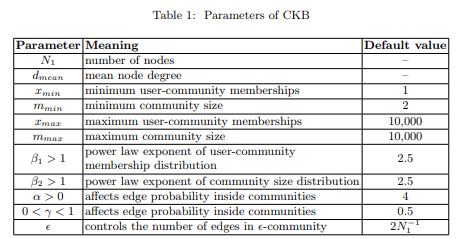
\includegraphics[width=0.6\textwidth]{ckb.PNG}
\caption{\label{fig:Parameters}Parameters used to generate graph}
\end{figure}



\subsubsection{Evaluation}
We use F1-score, precision and recall as metrics to evaluate the performance of the algorithms. Precision is the fraction of correctly classified vertices in the community and recall is the ratio of the number of correctly classified vertices to the total number of vertices that should be agglomerated into the community.
F1-score id the harmonic mean of precision and recall.

\[
F= 2 \times \frac{\text{Precision} \times \text{Recall}}{\text{Precision} + \text{Recall}}
\]


\subsubsection{Results}

The community is predicted using above algorithms around seed nodes. The predicted community's F-score is calculated with the ground truth communities. The following table displays the results calculated with bloom filter size = $3500$.
 

\begin{center}
\captionof{table}{Experiment 1 (100,000 nodes)}  
 \begin{tabular}{||c c c c c c c||} 
 \hline
 Algorithm & k & Memory(MB) & Precision & Recall & F-Score & Time(ms)\\ [0.4ex] 
 \hline\hline
 
 Page Rank Nibble & - & 60.78 & 0.06 & 0.16 & 0.05  & 35.31\\ 
 \hline
 LFM & - & 60.78 & 0.6 & 0.11 & 0.05 & 1,298.02\\ 
 \hline
 GCE & - & 937.45 & 0 & 0.33 & 0 & \\ 
 \hline
 GCE Local & - & 206.59 & 0.55 & 0.59 & 0.52 & 385.42\\ 
 \hline
 1 Node Expansion & - & 1.11 &0.58 & 0.54 & 0.53 & 1,416.47\\
 \hline
 Randomized with Lists & 20 & 1.13 & 0.67 & 0.29 & 0.40  & 409.57\\
 \hline
 Randomized with Lists & 30 & 1.12 & 0.81 & 0.42 & 0.5 & 214.49 \\
 \hline
 Randomized with Lists & 40 & 1.14 & 0.64 & 0.44 & 0.51  & 854.58 \\  
 \hline
 Randomized with Bloom Filter & 20 & 0.89 & 0.80 & 0.37 & 0.50 & 221,855.68\\  
 \hline
 Randomized with Bloom Filter & 30 & 0.89 & 0.65 & 0.40 & 0.48  & 265,731.79\\  
 \hline
 Randomized with Bloom Filter & 40 & 0.89 & 0.80 & 0.42 & 0.55  & 203,679.22\\  
 \hline
\end{tabular}
\end{center}



 We also studied variation of F1-score, precision recall and community size with change in $\alpha$. The results are summarized in figures 6 and 7. For these experiments, the same CKB generated graph of $100,000$ was used and the size of Bloom Filter was set to $200,000$.

\begin{figure}[h!]
    \centering
    \begin{minipage}{0.45\textwidth}
        \centering
       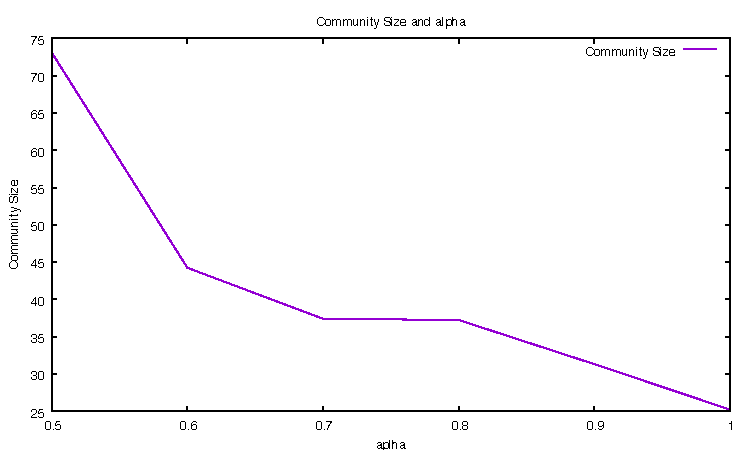
\includegraphics[width=1\textwidth]{CommunitySize.pdf}
\caption{\label{fig:Community Size and $\alpha$}Community Size and $\alpha$}
    \end{minipage}\hfill
    \begin{minipage}{0.45\textwidth}
        \centering
       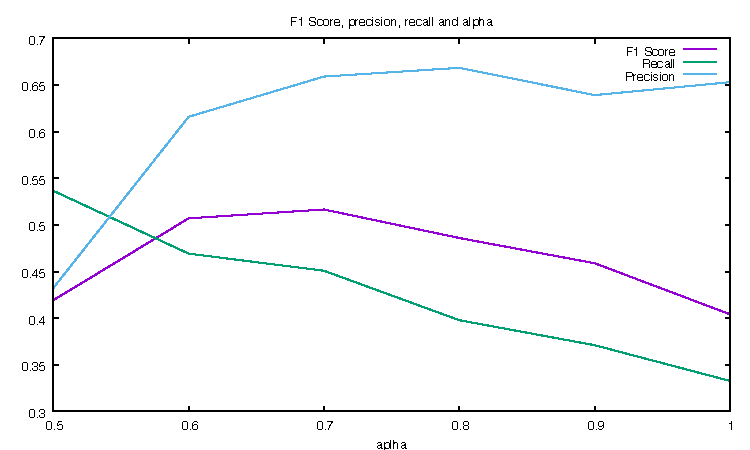
\includegraphics[width=1\textwidth]{40.pdf}
\caption{\label{fig:F1 Score, precision, recall and $\alpha$}F1 Score, precision, recall and $\alpha$}
    \end{minipage}
\end{figure}





\clearpage
\bibliographystyle{alpha}
\bibliography{sample}
\end{document}